\documentclass[twoside]{projektInzynierskiMS1}
\usepackage{polski}
\usepackage[utf8]{inputenc}
\usepackage{amsmath}
\usepackage{graphicx}%obrazki
\usepackage{array,etoolbox}%indeksowanie wierszy w tabelach
\preto\tabular{\setcounter{magicrownumbers}{0}}
\newcounter{magicrownumbers}
\newcommand\rownumber{\stepcounter{magicrownumbers}\arabic{magicrownumbers}}
\usepackage{multirow,tabularx}
\usepackage{etoolbox}
\newcounter{rowcnt}
\newcommand\rownum{\ifnumequal{\value{rowcnt}}{0}{\textbf{Nr.}}{\therowcnt.}\refstepcounter{rowcnt}}
\AtEndEnvironment{tabularx}{\setcounter{rowcnt}{0}}



%\drukJednostronny

%% tytuł promotor iautor (\title to komenda standardowa)
\title{Porównanie wybranych algorytmów heurystycznych w rozwiązywaniu zagadnień odwrotnych}
\promotor{dr inż. Adam Zielonka}


%% każdy autor musi mieć 3 argumenty: imię nazwisko, nr albumu, opis wkładu
\autor{Kamil Kryus}{246591}
	


%Custom commands
%-------------------------------------------------------------------------------
\newcommand{\hugeFontSize}{}
\newcommand{\newLine}{~\\}
\newcommand{\si}{ś}
\newcommand{\SI}{Ś}
%-------------------------------------------------------------------------------
%end Custom commands




%\NumeryNaPoczatku
%% numeracja wzorów tu włączona typu (1.2.3), ta druga to typu (1.2), domyślnie typu (1)
%\subsectionWzory
% \sectionWzory  

%\rozdzialy


%\literowaNumeracjaDodatkow %% włączy numerację dodatków literami
%\rzymskaNumeracjaDodatkow  %%włączy numerację dodatków liczbami rzymskimi

%% wyłączenie wyjaśnień:
\bezWyjasnien

%% standardowe komendy \newtheorem  działają jak woryginale
\newtheorem{tw}{Twierdzenie}%[subsection]
\newtheorem{twa}{Twierdzenie}%[section]
\newtheorem{dd}{Definicja}%[subsection]

\begin{document}




Na problem znalezienia optymalnego rozwiązania możemy trafić w wielu dziedzinach życia i nauki, np. w matematyce szukając globalnego minimum/maximum lub szukając najkrótszego połączenia pomiędzy kilkoma miastami (problem komiwojażera). Szukając rozwiązań, zawsze chcemy by było ono jak najlepsze (lub dokładnie najlepsze) i zostało znalezione w rozsądnym czasie. W tym celu wła\si nie jest używana heurystyka.\\ 


Metody heurystyczne znacznie skracają czas wyszukiwania rozwiązania problemu, aczkolwiek często ich wynikiem jest jedynie wynik bardzo zbliżony do najlepszego. Pozwala jednak nam to na jedną z dwóch rzeczy:
\begin{enumerate}
	\item zaakceptowanie takiego wyniku, gdy dokładne rozwiązanie nie jest konieczne (np. kompresja obrazu),
	\item zawężenia zakresu i dalszych poszukiwań najlepszego rozwiązania. \\
\end{enumerate}
Jednak aby metodę heurystyczną uznać za dobrą, musi ona spełniać 3 wymagania:
\begin{itemize}
	\item[--] rozwiązanie jest możliwe do znalezienia z rozsądnym wysiłkiem obliczeniowym,
	\item[--] rozwiązanie powinno być bliskie optymalnemu,
	\item[--] prawdopodobieństwo uzyskania złego rozwiązania powinno być niskie.
\end{itemize}

\section{Opis problemu}


Tu jest wnętrze rozdziału.

\begin{twa}
Twierdzenie Twierdzenie Twierdzenie Twierdzenie Twierdzenie 
\end{twa}
\begin{dd}
Twierdzenie Twierdzenie Twierdzenie Twierdzenie Twierdzenie 
\end{dd}

\thesection,\thesubsection,\thesubsubsection,

\subsection{Tytuł podrozdziału}
Francuzów sto wozów sieci purpurowe kwiaty każdy mimowolnie porządku pilnował
\begin{equation}
a^2+b^2=c^2.
\end{equation}

\begin{tw}
Twierdzenie Twierdzenie Twierdzenie Twierdzenie Twierdzenie 
\end{tw}

\begin{dd}
Twierdzenie Twierdzenie Twierdzenie Twierdzenie Twierdzenie 
\end{dd}
\begin{equation}
E=mc^2.
\end{equation}
\subsection{Cel}
	Przetestowanie algorytmu wyżarzania, bla bla 
pomimo, ze najlepiej sprawdza sie w zadaniach kombinatorycznych, to jak bedzie dzialac przy szukaniu minimum globalnym i zadaniach odwrotnych


\section{Opis algorytmów}
	\subsection{Algorytm symulowanego wyżarzania}
				Algorytm ten został stworzony wzorując się na zjawisku wyżarzania w metalurgii, które polega na nagrzaniu elementu stalowego do odpowiedniej temperatury, przetrzymaniu go w tej temperaturze przez pewien czas, a następnie powolnym jego schłodzeniu. Sam algorytm natomiast bazuje na metodach Monte-Carlo i w pewnym sensie może być rozważany jako algorytm iteracyjny.\\ \newLine
Główną istotą i zarazem zaletą tego algorytmu jest wykonywanie pewnych losowych przeskoków do sąsiednich rozwiązań, dzięki czemu jest w stanie uniknąć wpadania w lokalne minimum. Algorytm ten najczę\si ciej jest używany do rozwiązywania problemów kombinatorycznych, jak np. problemu komiwojażera.
		\subsubsection{Parametry}
		


\noindent \underline{Początkowa konfiguracja} \\ \newLine
\indent W tym kroku powinniśmy zainicjalizować naszą temperaturę wysoką wartością oraz znaleźć początkowe losowe rozwiązanie naszego problemu. 
\\ \newLine

\noindent \underline{Temperatura} \\ \newLine
\indent Temperatura jest zarówno czynnikiem iteracyjnym, jak i jest związana z funkcją prawdopodobieństwa zamiany gorszego rozwiązania na lepsze. Zatem zakres temperatury powinien być taki, aby na początku działania naszego algorytmu dawał wysoką możliwość zamian, a wraz z postępem iteracji te prawdopodobieństwo się zmniejszało i pod koniec było bliskie zeru.\\ \newLine


\noindent \underline{Końcowa temperatura} \\ \newLine
\indent Jest to bardzo mała wartość. Temperatura osiągając taki poziom informuje nas iż proces wyżarzania się zakończył i rozwiązanie zostało znalezione.
Wartość ta powinna być na tyle mała, by temperatura będąc niewiele większa prowadziła do bardzo niskiego prawdopodobieństwa, a jednocze\si nie nie wymagało to zbyt dużej ilo\si ci iteracji. \\ \newLine


\noindent \underline{Powtarzanie pewną ilość razy dla zadanej temperatury} \\ \newLine
\indent Wartość ta powinna być z góry ustalona i powinna dać nam możliwość sprawdzenia wielu sąsiadów obecnego rozwiązania, równocześnie nie powodując zbyt dużego obciążenia dla algorytmu.\\ \newLine


\noindent \underline{Znajdowanie losowego sąsiada poprzedniego rozwiązania} \\ \newLine
\indent Funkcja ta powinna nam pozwalać przejrzeć jak najszerszy zakres rozwiązań, a jednocze\si nie pozwolić na przeszukiwanie coraz to bliższych sąsiadów obecnie najlepszego rozwiązania, zatem warto uzależnić tą funkcję od stopnia ukończenia globalnych iteracji.\\ \newLine


\noindent \underline{Funkcja kosztu} \\ \newLine
\indent Poprzez funkcję kosztu rozumiemy różnicę pomiędzy obecnie najlepszym rozwiązaniem, a nowym. Przy poszukiwaniu globalnego minimum warto\si ć większa jest gorszym rozwiązaniem, dzięki czemu wynikiem tej funkcji jest zawsze liczba ujemna.
 W tym wypadku nowe rozwiązanie zawsze jest gorsze (a tym samym przy poszukiwaniu minimum globalnego posiada warto\si ć większą), to w tym wypadku warto\si ć jest ujemna.\\ \newLine


\noindent \underline{Prawdopodobieństwo zamiany P} \\ \newLine
\indent Prawdopodobieństwo jest potrzebne do decyzji czy zamienić nasze nowe i gorsze rozwiązanie z wcze\si niejszym, lepszym. 

Prawdopodobieństwo zależy od funkcji kosztu oraz obecnej temperatury. Prawdopodobieństwo zatem można przedstawić w następujący sposób:
\[P = e^\frac{\Delta E}{T} \]
gdzie:\\
\begin{flalign}
& \Delta E - funkcja\ kosztu& 
\end{flalign}
T - obecna warto\si ć temperatury\\

Prawdopodobieństwo to wraz ze spadkiem warto\si ci funkcji kosztu maleje (gdyż jest zawsze ujemne), natomiast wyższa warto\si ć temperatury zwiększa prawdopodobieństwo. Decydując o tym czy powinniśmy zamienić nasze gorsze rozwiązanie z lepszym powinniśmy porównać obliczone prawdopodobieństwo z wartością losową zawierającą się w zakresie [0,1].\\ \newLine


\noindent \underline{Zmniejszanie temperatury} \\ \newLine
\indent Szybkość zmniejszania nie powinna być zbyt duża, aby pozwolić algorytmowi na sprawdzenie jak największego zakresu możliwych rozwiązań, a jednocześnie niezbyt wolna, gdyż może to spowodować zbyt wolny spadek prawdopodobieństwa, a tym samym finalnie pozwolić na pozostanie w gorszym rozwiązaniu. W większości opracowań można spotkać ten proces, jako mnożnik temperatury w zakresie [0.8;0.99].\\ \newLine
		
		\subsubsection{Kroki algorytmu}
		
		Algorytm ten można również przedstawić za pomocą listy kroków:

\begin{enumerate}
	\item Zainicjalizuj początkową konfigurację
	\item Dopóki temperatura > minimum, powtarzaj:
	\begin{enumerate}
		\item Powtórz pewną ilość razy dla danej temperatury
		\begin{enumerate}
			\item Znajdź losowo sąsiada poprzedniego rozwiązania
			\item Sprawdź czy rozwiązanie jest lepsze od poprzedniego (funkcja kosztu)
			\begin{enumerate}
				\item Jeżeli jest, zamień rozwiązania
				\item Jeżeli nie jest, zamień rozwiązania z pewnym prawdopodobieństwem P
			\end{enumerate}
		\end{enumerate}
		\item Zmniejsz temperaturę
	\end{enumerate}
\end{enumerate}
		

\section{Funkcje testowe}
	\subsection{Funkcja kwadratowa dwóch parametrów}
	Funkcja ta ma następującą postać:

\[f(x, y) = x^2 + y^2 \]

Co\si o wykresie:\\
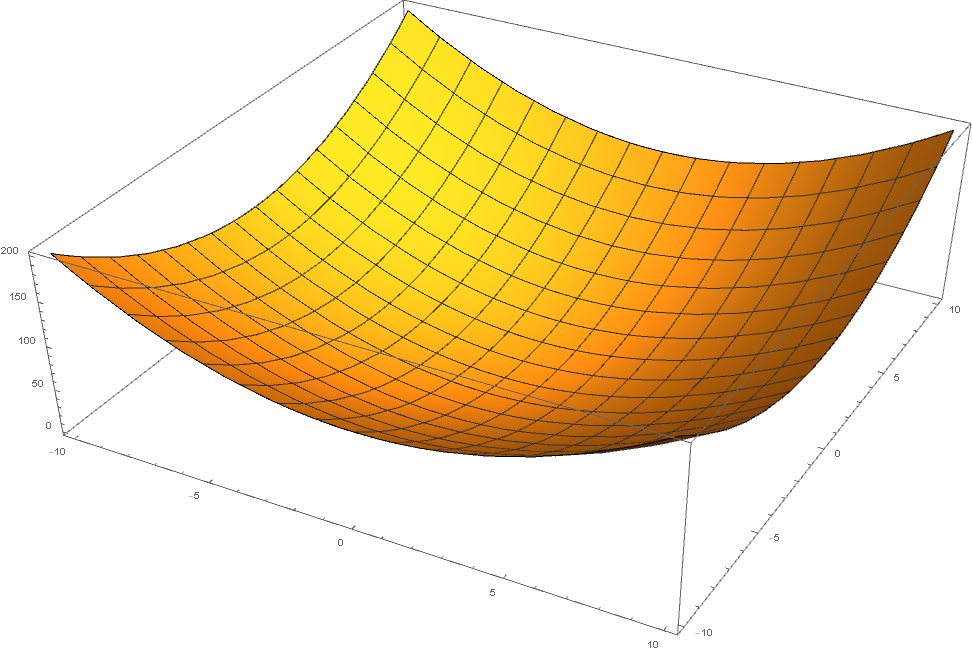
\includegraphics[height=8cm]{quadraticFunction1.png}\\
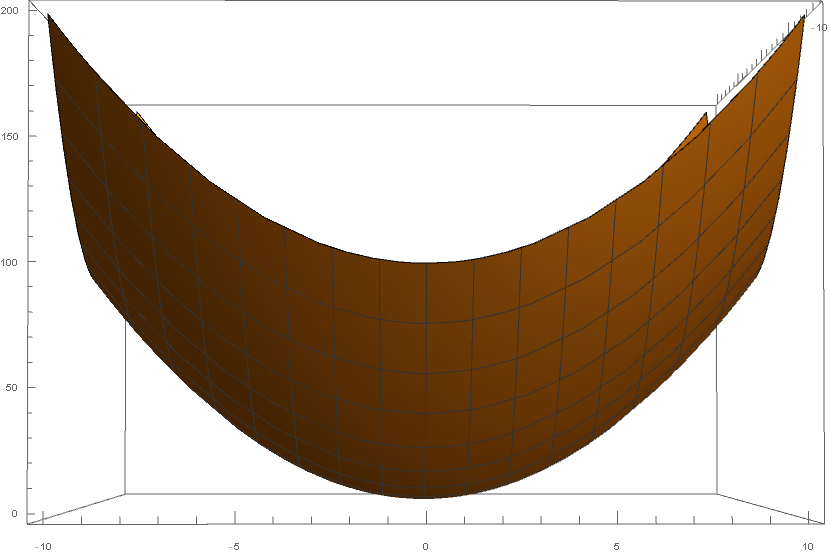
\includegraphics[height=8cm]{quadraticFunction2.png}\\
<tutaj jakis wykres >

Funkcja ta przyjmuje jedynie warto\si ci dodatnie, zakres dla potrzeb projektu został zawężony do [-10, 10], natomiast minimum globalne posiada w punkcie [0, 0] i wynosi 0. 
	\subsection{Funkcja Rastrigina}
	Funkcja Rastrigina jest funkcją ciągłą, skalowalną i multimodalną. Dzięki posiadaniu wielu minimum lokalnych funkcja ta jest często stosowana w testowaniu algorytmów optymalizacyjnych. 

\[f(x) = An + \sum_{i=1}^{n} [x_i^2 - A \cos{(2 \pi x_i)}] \]

gdzie: \\
A = 10, \\
n = ilo\si ć wymiarów \\ \newLine

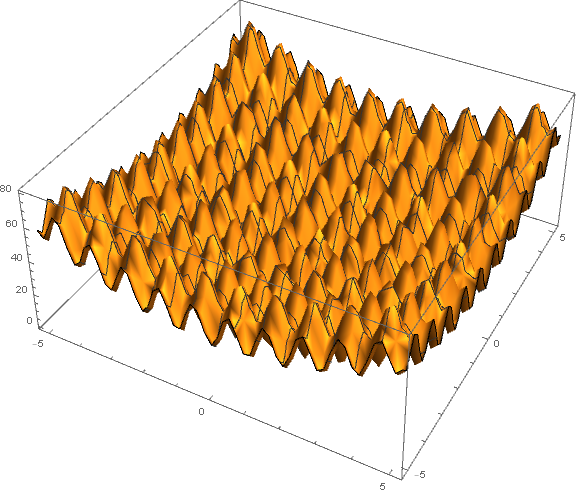
\includegraphics[height=8cm]{rastriginFunction1.png}\\
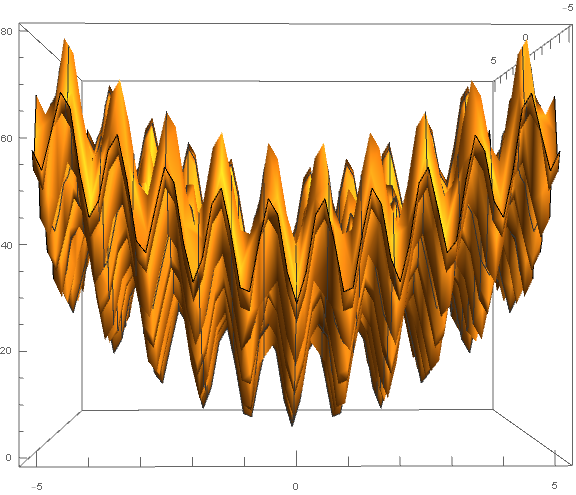
\includegraphics[height=8cm]{rastriginFunction2.png}\\


Parametry funkcji możemy znaleźć w zakresie [-5.12; 5.12], minimum globalne natomiast w punkcie [0,...,0] i wynosi 0.
	\subsection{Funkcja Rosenbrocka}
	Rosenbrock's valley function is known as the second function of De Jong. This test function is continuous, scalable, naturally nonseparable, nonconvex, and unimodal.


\[f(x) = \sum_{i=1}^{n-1} [100(x_{i+1} - x_i^2)^2 + (1- x_i)^2 ]\]

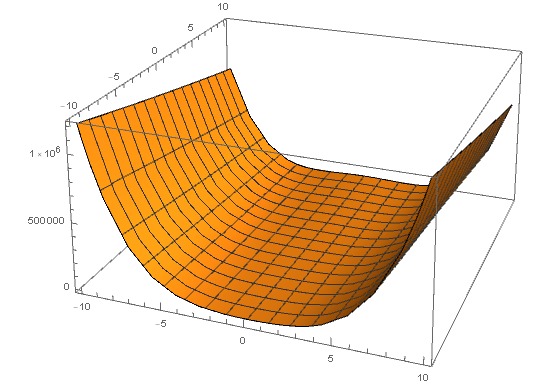
\includegraphics[height=8cm]{rosenbrockFunction1.png}\\
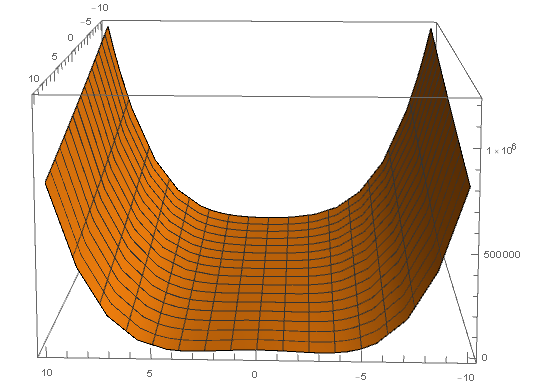
\includegraphics[height=8cm]{rosenbrockFunction2.png}\\

\section{Dobór parametrów}
Pomimo, iż algorytmy heurystyczne są dobrym wyborem wszędzie tam, gdzie ważny jest czas znalezienia rozwiązania, to przed skorzystaniem z danego algorytmu jeste\si my zmuszeni ustawić parametry algorytmu w taki sposób, by wynik był dostatecznie dokładny, a algorytm nie wykonywał niepotrzebnie obliczeń, zwłaszcza gdy większa dokładno\si ć nie jest nam potrzebna lub nie będzie stanowić większej różnicy w stosunku do już znalezionego wyniku. Dodatkową trudno\si ć stanowi ilo\si ć parametrów oraz to, iż każdy z nich może wpływać w inny sposób na złożono\si ć obliczeniową oraz wynik, oraz parametry mogą być od siebie zależne. W opracowaniach naukowych rzadko kiedy można znaleźć wytyczne co do sposobu znalezienia odpowiednich parametrów do konkretnych problemów. \\

Starając się trzymać zasad dotyczących tworzenia dobrego algorytmu heurystycznego, przyjąłem kilka założeń, a następnie sukcesywnie poszukiwałem odpowiednich warto\si ci dla parametrów by (\si redni, 10-krotne powtórzenia) wynik był jak najlepszy, starając się zawężać zakres z czasem. Kiedy (\si rednie) wyniki były już zadowalające, sprawdzałem jako\si ć dobranych parametrów wykonując 100 razy algorytm z takimi samymi parametrami dla tego samego problemu, uzysując w prosty sposób procentową jako\si ć algorytmu. W podsekcji "Dobieranie parametrów dla funkcji 5 wymiarowej funkcji Rastrigina" tabele przedstawią stopniowe doj\si cie do parametrów dających zadowalające wyniki, a następnie jako\si ć tych parametrów dla danego problemu. Parametry dla innych problemów zostały zbadane w taki sam sposób i w tych sekcjach zostanie wspomniany jedynie wynik.

	\subsection{Dobieranie parametrów dla funkcji 5 wymiarowej funkcji Rastrigina}

Przed rozpoczęciem testów przyjęto dwa założenia:
\begin{enumerate}
	\item Końcowa temperatura została ustawiona na stałą warto\si ć równą 0.001,
	\item Stopień chłodzenia temperatury został ustawiony na 0.99.
\end{enumerate}

\renewcommand\arraystretch{1.333}
\begin{tabularx}{\textwidth}{ | >{\rownum}c|X|X|X|}
  \hline
    & \textbf{T0} & \textbf{Iteracje} &\textbf{Rozwiązanie}\\ \hline
    & aaaaaaa aaaaaaa & aaaaaaa aaaaaaa  & oko\\ \hline
    & aaaaaaa aaaaaaa &aaaaaaa & oko \\ \hline
    & aaaaaaa & aaaaaaaaaaaaaa & oko \\ \hline
 & aaaaaaa & aaaaaaaaaaaaaa & oko \\ \hline
 & aaaaaaa & aaaaaaaaaaaaaa & oko \\ \hline
 & aaaaaaa & aaaaaaaaaaaaaa & oko \\ \hline
 & aaaaaaa & aaaaaaaaaaaaaa & oko \\ \hline
 & aaaaaaa & aaaaaaaaaaaaaa & oko \\ \hline
 & aaaaaaa & aaaaaaaaaaaaaa & oko \\ \hline
 & aaaaaaa & aaaaaaaaaaaaaa & oko \\ \hline
 & aaaaaaa & aaaaaaaaaaaaaa & oko \\ \hline
 & aaaaaaa & aaaaaaaaaaaaaa & oko \\ \hline

\end{tabularx}

\begin{tabularx}{\textwidth}{ | >{\rownum}c|X|X|X|}
  \hline
    & \textbf{T0} & \textbf{Iteracje} &\textbf{Rozwiązanie}\\ \hline
    & aaaaaaa aaaaaaa & aaaaaaa aaaaaaa  & oko\\ \hline
    & aaaaaaa aaaaaaa &aaaaaaa & oko \\ \hline
    & aaaaaaa & aaaaaaaaaaaaaa & oko \\ \hline
 & aaaaaaa & aaaaaaaaaaaaaa & oko \\ \hline
 & aaaaaaa & aaaaaaaaaaaaaa & oko \\ \hline
 & aaaaaaa & aaaaaaaaaaaaaa & oko \\ \hline
 & aaaaaaa & aaaaaaaaaaaaaa & oko \\ \hline
 & aaaaaaa & aaaaaaaaaaaaaa & oko \\ \hline
 & aaaaaaa & aaaaaaaaaaaaaa & oko \\ \hline
 & aaaaaaa & aaaaaaaaaaaaaa & oko \\ \hline
 & aaaaaaa & aaaaaaaaaaaaaa & oko \\ \hline
 & aaaaaaa & aaaaaaaaaaaaaa & oko \\ \hline

\end{tabularx}


\begin{tabularx}{\textwidth}{ | >{\rownum}c|X|X|X|}
  \hline
    & \textbf{T0} & \textbf{Iteracje} &\textbf{Rozwiązanie}\\ \hline
    & aaaaaaa aaaaaaa & aaaaaaa aaaaaaa  & oko\\ \hline
    & aaaaaaa aaaaaaa &aaaaaaa & oko \\ \hline
    & aaaaaaa & aaaaaaaaaaaaaa & oko \\ \hline
 & aaaaaaa & aaaaaaaaaaaaaa & oko \\ \hline
 & aaaaaaa & aaaaaaaaaaaaaa & oko \\ \hline
 & aaaaaaa & aaaaaaaaaaaaaa & oko \\ \hline
 & aaaaaaa & aaaaaaaaaaaaaa & oko \\ \hline
 & aaaaaaa & aaaaaaaaaaaaaa & oko \\ \hline
 & aaaaaaa & aaaaaaaaaaaaaa & oko \\ \hline
 & aaaaaaa & aaaaaaaaaaaaaa & oko \\ \hline
 & aaaaaaa & aaaaaaaaaaaaaa & oko \\ \hline
 & aaaaaaa & aaaaaaaaaaaaaa & oko \\ \hline

\end{tabularx}

Ostatecznie wybrane parametry dla tego problemu:\\
pocz temp\\
konc temp\\
cooling\\
iteracje\\

Badanie skutecznosci \\






skutecznosc:\\






	\subsection{Dobieranie parametrów dla funkcji 3 wymiarowej funkcji Rastrigina}
Ostatecznie wybrane parametry dla tego problemu:\\
pocz temp\\
konc temp\\
cooling\\
iteracje\\






skutecznosc:\\


	\subsection{Parametry dobrane dla funkcji kwadratowej dwóch parametrów}
Ostatecznie wybrane parametry dla tego problemu:\\
pocz temp\\
konc temp\\
cooling\\
iteracje\\






skutecznosc:\\

	\subsection{Parametry dobrane dla funkcji Rosenbrocka}
Ostatecznie wybrane parametry dla tego problemu:\\
pocz temp\\
konc temp\\
cooling\\
iteracje\\






skutecznosc:\\

\section{Implementacja}
\section{Dostosowanie algorytmów do funkcji testowej zadań odwrotnych}
\section{Narzędzia i technologie}
	\subsection{Użyte narzędzia}
	Aby zapewnić bezpieczeństwo oraz możliwo\si ć pracy w kilku miejscach nad jednym problemem, zastosowałem kilka rozwiązań.
	\subsubsection{System kontroli wersji}
	Git
	\subsubsection{Podział pracy na mniejsze zadania}
	Git
	\subsection{Użyte technologie}
	.NET Framework \\
Ponadto wykresy zawarte w dokumentacji są stworzone z pomocą programu Mathematica używanego na licencji Wydziału Matematyki Stosowanej.

b labla
\section{Podsumowanie}
	\subsection{Dalsze kierunki rozwoju}
	\subsection{Źródła}
%funkcje testowe
https://www.ncbi.nlm.nih.gov/pmc/articles/PMC4538776/

%wstep i opis problemu[?]
F. Rothlauf, Design of Modern Heuristics, Natural Computing Series,
DOI 10.1007/978-3-540-72962-4 2, © Springer-Verlag Berlin Heidelberg 2011

%wstep i opis problemu
R. Mart'ı and G. Reinelt, The Linear Ordering Problem, Exact and Heuristic Methods
in Combinatorial Optimization 175, DOI: 10.1007/978-3-642-16729-4 2,
c Springer-Verlag Berlin Heidelberg 2011


----------------------------------------------------------------------------------------------------------------------
%% UWaga na \newlineTekst oraz \newlineSpis. Można też użyć \newline, działa jak \newlineSpis\newlineTekst
\section[Tytuł drugiego rozdziału. Bardzo długi \ldots]
        {Tytuł drugiego rozdziału. \newlineTekst Bardzo długi tytuł. \newlineTekst
          Jego \newlineSpis formatowanie jest trudniejsze}



\dodatek{Mój specjalny dodatek}

Tu treść dodatku. Zwróćmy uwagę na sposób numerowania dodatku, 
możliwa jest zmiana numerowania, patrz wyjaśnienia.
          
%% to wpisuje się do spisu treści, ale bez numeru rozdziału,
%% można też używać \dodatek{Tytuł}, który jest numerowany, ale inaczej niż rozdziały.
\dodatkowo{Rysunki}

Tu rysunki

\dodatkowo{Programy}

Tu programy

\begin{verbatim}
#include <stdio.h>

int main()
{
   printf("Hello world\n");
}
\end{verbatim}

\noindent
Oraz 

\bigskip

\vrule\hspace{10pt}\begin{minipage}{10cm}
\begin{verbatim*}
<?php
   echo "test=$test";
?>
\end{verbatim*}
\end{minipage}

\begin{tw}
Twierdzenie Twierdzenie Twierdzenie Twierdzenie Twierdzenie 
\end{tw}
\begin{thebibliography}{12}

\bibitem{PozNazwa1} Jakaś pozycja literatury
\bibitem{InnPoz} Jakaś pozycja literatury

\end{thebibliography}
\end{document}
